\documentclass[UTF8,12pt,a4paper]{ctexart}

\usepackage{amsmath}
\usepackage{cases}
\usepackage{cite}
\usepackage{graphicx}
\usepackage{enumerate}
\usepackage{caption} %\caption*需要
\usepackage[noend]{algpseudocode} %algorithmicx
\usepackage[margin=1in]{geometry}
\geometry{a4paper}
\usepackage{fancyhdr}
\pagestyle{fancy}
\fancyhf{}
\usepackage{xcolor}
\usepackage{listings}
\usepackage{float}
\usepackage{hyperref}
\lstset{
	basicstyle=\ttfamily,                                % 传统上,代码打字机字体好些
	breaklines,
	tabsize=4,
	extendedchars=false,
	columns=fixed,
	%numbers=left,                                        % 在左侧显示行号
	numbers=none,
	frame=none,                                          % 不显示背景边框
	backgroundcolor=\color[RGB]{245,245,244},            % 设定背景颜色
	keywordstyle=\color[RGB]{40,40,255},                 % 设定关键字颜色
	numberstyle=\footnotesize\color{darkgray},           % 设定行号格式
	commentstyle=\it\color[RGB]{0,96,96},                % 设置代码注释的格式
	stringstyle=\rmfamily\slshape\color[RGB]{128,0,0},   % 设置字符串格式
	showstringspaces=false,                              % 不显示字符串中的空格
	xleftmargin=1em,
	%xrightmargin=1em,
	%aboveskip=-0.5em
	language=c++,                                        % 设置语言
}
\hypersetup{hidelinks,
	colorlinks=true,
	allcolors=purple,
	pdfstartview=Fit,
	breaklinks=true}
\usepackage[vlined,ruled,linesnumbered]{algorithm2e}


\title{基于神经网络的高血压视网膜分类}
\author{金天宇、林袁艺、廖凡 }
\date{\footnotesize
\href{https://github.com/PressurePoints/CS3511-CodaLab-Hypertensive-Retinopathy-Diagnosis-Challenge}{https://github.com/PressurePoints/CS3511-CodaLab-Hypertensive-Retinopathy-Diagnosis-Challenge}
}
\pagenumbering{arabic}

\begin{document}

\fancyhead[L]{金天宇、林袁艺、廖凡}
\fancyhead[R]{HRDC}
\fancyfoot[C]{\thepage}

\maketitle
%\tableofcontents
%\newpage


\section{摘要}
高血压视网膜病变是高血压在眼部的主要表现,早期发现和诊断对于预防和控制高血压及其并发症具有
重要意义。本文基于 HRDC(Hypertensive Retinopathy Diagnosis Challenge,高血压视网膜病变诊断挑战)
提供的高血压视网膜病变数据集,探索了使用深度学习算法进行高血压视
网膜病变分类的方法。本小组尝试了不同的数据预处理方法和深度学习模型,寻找最合适对高血压视网
膜病变分类的方法。

\textbf{关键词:}高血压视网膜病变;二分类问题;数据预处理

\section{简介与意义}
\subsection{项目背景}
高血压视网膜病变是高血压在眼部的主要表现,早期发现和诊断对于预防和控制高血压及其并发症具有
重要意义。然而,传统的视网膜病变诊断主要依赖于医生的经验和视觉判断,这种方式不仅耗时耗力,
而且容易受到主观因素的影响,导致诊断的准确性和一致性受限。因此,研究并开发一种计算机辅助
临床自动诊断系统,用于高血压视网膜病变的筛查和诊断,成为当前医学和计算机科学领域的研究热点。
通过应用机器学习和深度学习算法,实现高血压视网膜病变的自动诊断,可以显著提高诊断的效率和
准确性,降低漏诊和误诊的风险。此外,这种自动诊断系统还可以为医生提供客观、量化的诊断依据,
有助于提升医疗服务的质量和水平。

尽管近年来机器学习和深度学习在医疗图像识别领域取得了显著进展,但在高血压视网膜病变自动诊断
方面仍面临一些技术困难和挑战。首先,视网膜图像的获取和处理涉及复杂的医学知识和图像处理技术,
需要跨学科的合作和深入研究。其次,高血压视网膜病变的病理特征多样且复杂,如何在海量数据中
提取有效特征并进行准确分类是一个难题。此外,由于数据标注的困难和标注质量的不一致性,如何
构建高质量的训练数据集也是一个需要解决的问题。
\subsection{方法框架}
为了完成任务 2: 高血压视网膜病变分类。给定患者眼睛的眼底图像,确认是否患有高血压性视网膜病变。
0 类代表无高血压性视网膜病变,1 类代表高血压性视网膜病变。这是一个两类分类任务。本小组使用了
机器学习和深度学习算法,实现在高血压视网膜病变计算机辅助临床自动诊断中的应用。为了充分提取
图片特征,首先对图片进行图像增强、去噪等数据预处理方法,通过直方图均衡算法 CLAHE 进行图像
增强,然后分别使用三个网络:简单卷积网络、 EfficientNetV2 和 ResNet 对图片进行预测,对它们
的结果进行投票得出最终的预测结果。方法流程如图 1 所示。
\begin{figure}[H]
	\centering
	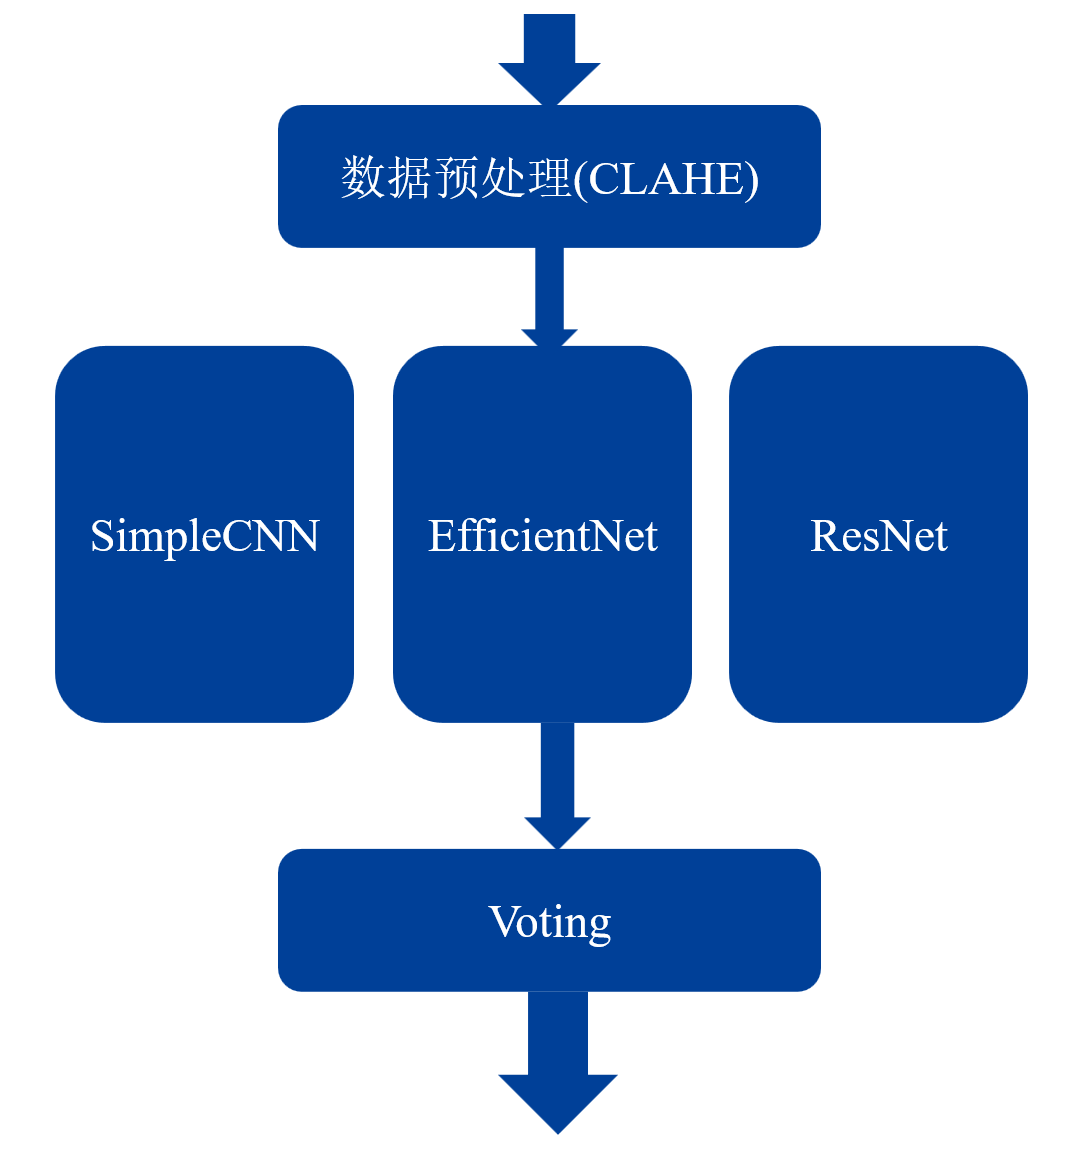
\includegraphics[width=0.6\textwidth]{picture/procedure.png}
	\caption{方法流程图}
\end{figure}


\section{相关工作}
\subsection{图像预处理}
为了让神经网络对图像更好地提取图片的特征,图像的预处理是至关重要的一环。
它旨在通过一系列的操作和技术对原始图像进行操作,以改善其质量、增强特征或准备用于
进一步的图像分析和识别任务。现在常用的图像预处理方法有:
\begin{itemize}
	\item \textbf{尺寸调整与裁剪}:将图像调整到指定的尺寸,或者根据需要进行裁剪以消除无关区域,
确保图像尺寸一致性。
	\item \textbf{灰度化}:将彩色图像转换为灰度图像,去除颜色信息,简化图像处理流程,并减少计算成本。
	\item \textbf{去噪}:消除图像中的噪声,例如高斯噪声、椒盐噪声等,以提高图像的清晰度和质量。常用的方法包括中值滤波、高斯滤波等。
	\item \textbf{直方图均衡化}:通过调整图像的像素强度分布,增强图像的对比度和亮度,使图像更加清晰和易于分析。
	\item \textbf{边缘检测}:检测图像中的边缘信息,突出物体的边界结构,常用的边缘检测算法包括 Sobel、Canny 等。
	\item \textbf{图像增强}:通过增强图像的局部特征或者整体特征,使图像更具有视觉吸引力或者更适合于
后续的分析任务。常见的增强方法包括对比度增强、锐化、颜色增强等。
	\item \textbf{几何校正}:校正图像中的几何变形或者失真,使图像更加符合实际场景,常用的校正方法
包括透视变换、仿射变换等。
	\item \textbf{图像去除}:移除图像中的不相关信息或者干扰因素,如水印、文本、阴影等,以提高图像的
纯净度和可用性。
	\item \textbf{数据增强}:通过对原始图像进行旋转、翻转、缩放等操作,生成更多样化的训练数据,增强
模型的泛化能力和鲁棒性。
\end{itemize}

这些方法常常结合使用,根据具体的任务和需求进行调整和组合,以达到更好的图像预处理效果。

\subsection{深度学习}
深度学习在医学领域的应用已经取得了许多令人振奋的成果,使用基于深度学习的方法
对医学图像进行分类可以极大地提高准确性,且具有很强的适应性。

在眼底图片分析方面,深度学习模型可通过眼底摄影获取的图像,用于诊断和监测多种眼部疾病,
如糖尿病视网膜病变、青光眼、黄斑变性等。深度学习模型能够学习并识别眼底图片中的病变特征,
如微血管瘤、出血斑点、渗出物等,从而帮助医生进行疾病的检测和诊断。例如,针对糖尿病视网膜
病变的检测,深度学习模型已经取得了很高的准确度。深度学习模型可以根据眼底图片中病变的
严重程度和分布情况,对患者的病情进行分级和评估,为医生提供更全面的诊断信息和治疗建议。
深度学习在眼底图片分析中的应用,不仅为医生提供了更精准的诊断工具,也为患者提供了更及时、
更有效的医疗服务,对促进眼部健康和预防眼部疾病具有重要意义。

\section{研究内容与算法}
\subsection{数据预处理}
本小组在数据预处理阶段主要采用了对比度受限自适应直方图均衡化(CLAHE)算法对图像进行
增强处理。它是一种简单快速的图像增强方法,主要用在医学图像上面。原理大致为通过将
原始图像的灰度
直方图划分成若干个子区域,对子区域分别进行受对比度限制的直方图均衡化,再利用双线性
差值消除各个子区域间比较明显的截断部分,得到一张对比度增强的图像。本文应用此处理方法
得到了病灶特点更明显的图片。
\begin{figure}[H]
	\centering
	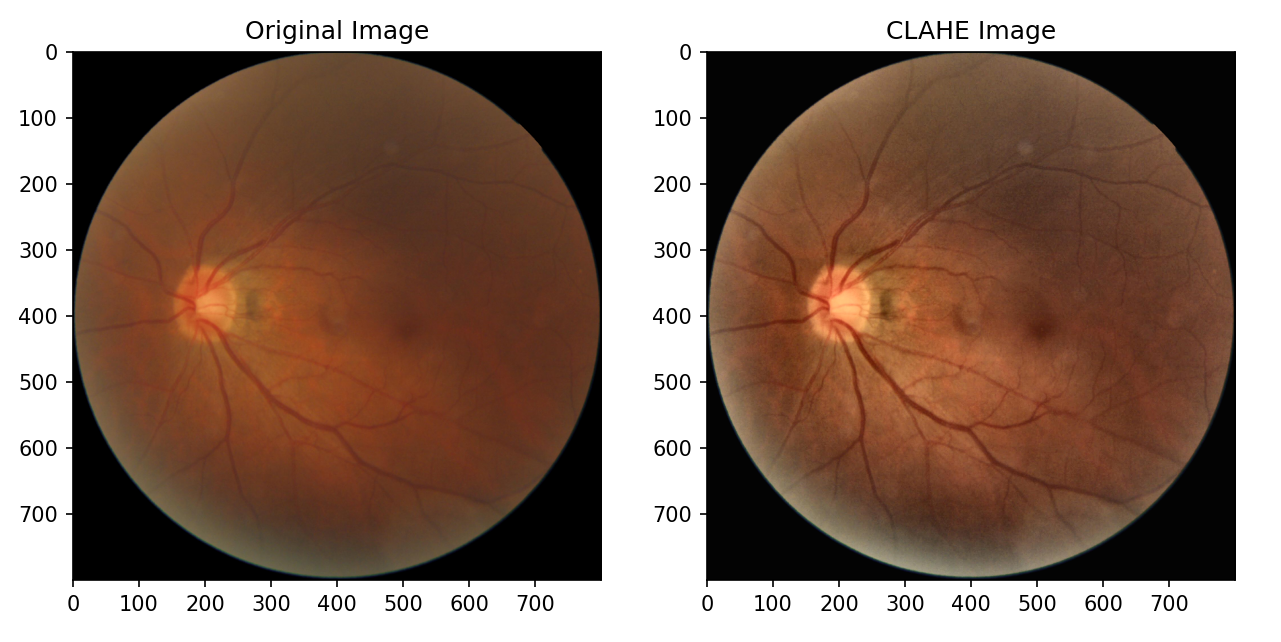
\includegraphics[width=0.6\textwidth]{picture/clahe.png}
	\caption{CLAHE 图像增强方法应用前后图片对比}
\end{figure}

训练模型所用的图片均来自 HRDC 提供的数据集,数据集中包含了 712 张眼底图片,其中包含
420 张正常眼底图片和 292 张高血压性视网膜病变图片。除了 CLAHE 算法外,
本小组还对图像进行了尺寸调整、灰度化、去噪等处理,以提高图像的质量和清晰度。
完整流程为:首先选择图像的绿色通道进行处理,然后对图像进行 CLAHE 处理,反转后再进行
一次 CLAHE 处理,然后使用中值滤波去除噪声,接着使用顶帽操作去除背景,最后将图像
调整为 64*64 大小的灰度图像,并将像素值归一化到 [0, 1] 区间。
\begin{figure}[H]
	\centering
	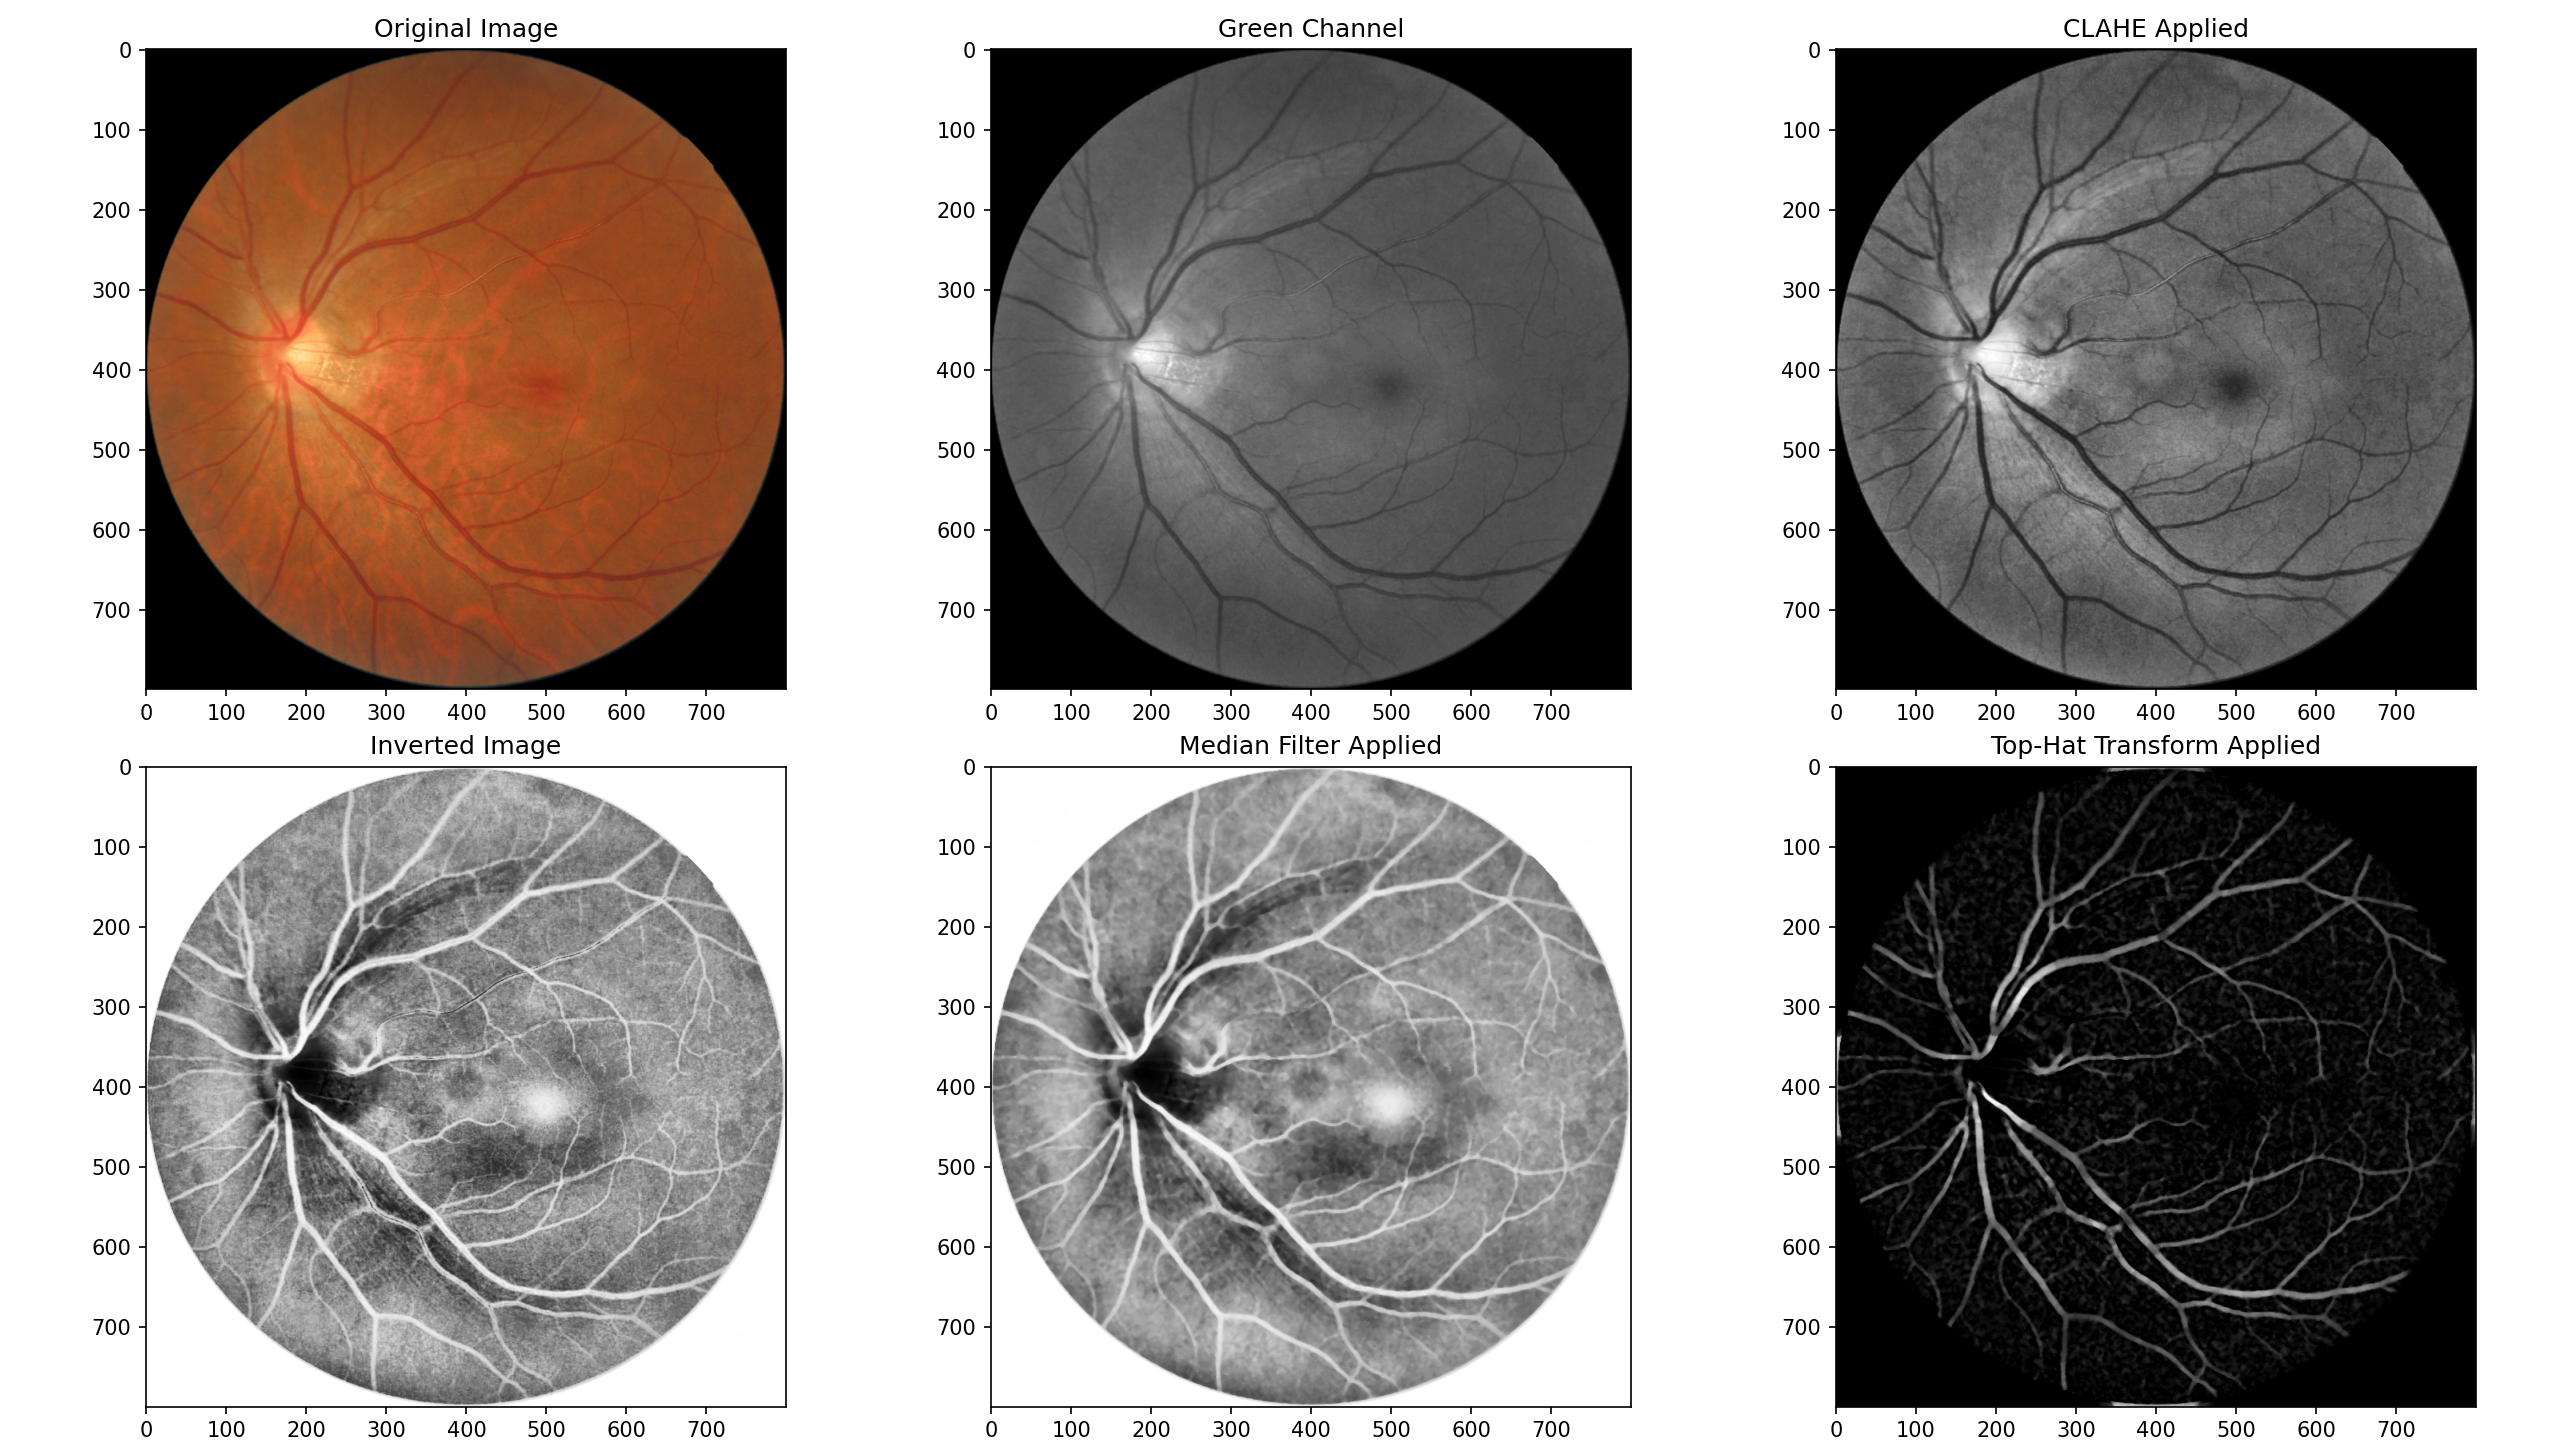
\includegraphics[width=0.6\textwidth]{picture/preprocess.png}
	\caption{数据预处理流程}
\end{figure}

在使用 EfficientNetV2 模型时,本小组还尝试了 CutMix 数据增强方法。CutMix 
作为一种数据增强方法,可以增加模型对于图像位置和内容的鲁棒性。具体过程为,
通过在两张随机选取的图像中剪切并交换一部分来生成新的训练数据,经过模型输出后,
将两张原始图像的标签按照剪切区域的面积加权平均来计算。
\subsection{模型设计}
\subsubsection{卷积神经网络}
卷积神经网络(ConvolutionalNeural Networks, CNN)是一类包含卷积计算且具
有深度结构的前馈神经网络(Feedforward Neural Networks),是深度学习(deep
 learning)的代表算法之一。主流的 CNN 模型包含卷积、非线性变换、池化和全连接层。

在选择深度学习的模型时,本小组首先设计了一个简单的卷积神经网络,包含三个卷积层、
三个池化层和两个全连接层。卷积层用于提取图像的特征,池化层用于降维和减少参数,
全连接层用于分类和输出预测结果。

为了了解模型的性能,本小组以 $7: 3$ 将数据集分为训练集和测试集,并采用二分类交叉熵
损失函数和 Adam 优化器进行模型训练,以准确率作为评价指标。
以下为本地训练模型的伪代码:

\begin{algorithm}[H]
	\caption{train.py}
	\BlankLine

	load $datasets$ and $labels$\;
	preprocess$(datasets)$\;
	$train\_datasets$, $test\_datasets$, $train\_labels$, $test\_labels$ = split$(datasets, labels)$\;
	$model$ = SimpleCNN()\;
	$optimizer$ = Adam()\;
	$loss\_fn$ = CrossEntropyLoss()\;
	$train\_loader$ = DataLoader($train\_datasets$, $train\_labels$)\;
	$test\_loader$ = DataLoader($test\_datasets$, $test\_labels$)\;
	\For{$epoch$ in $range(epochs)$}{
		\For{$batch$ in $train\_loader$}{
			$optimizer.zero\_grad()$\;
			$preds$ = $model(batch)$\;
			$loss$ = $loss\_fn(preds, labels)$\;
			$loss.backward()$\;
			$optimizer.step()$\;
		}
		$acc$ = evaluate($model$, $test\_loader$)\;
		print($epoch$, $loss$, $acc$)\;
	}
\end{algorithm}

\subsubsection{ResNet}
ResNet,即深度残差网络(Residual Network),通过引入残差模块(residual module)
来解决深度神经网络训练过程中的梯度消失和梯度爆炸问题。利用残差学习(residual learning),
即学习输入和输出之间的残差(即差值),而不是直接学习输出值。避免网络深度增加时的性能退化
问题,同时减轻了训练难度。ResNet 最常用的版本是通过堆叠残差模块来构建网络,其中每个残差模块
包含两个具有相同输出特征图大小的卷积层,以及一个跳跃连接。

于是本小组采用的网络结构,在 Resnet 后接全连接层,首先经 Linear 层将原网络生成的结果向量统一
为 256 大小,然后经 ReLU 后设置一个 Dropout 单元,参数设置 0.3,最后将向量降至 2 维,输出预测结果。

\subsubsection{EfficientNetV2}
EfficientNetV2 作为一个知名的卷积神经网络,以训练速度快,参数量少,精度高,
泛化性能强为特点。原论文中给出了此网络与其他著名网络的准确率和性能时间对比,
如下图。不难看出,EfficientNetV2 网络在准确率,训练时间上都显著优于 ResNet-RS,
botnet,lambdanet 等网络。
\begin{figure}[H]
	\centering
	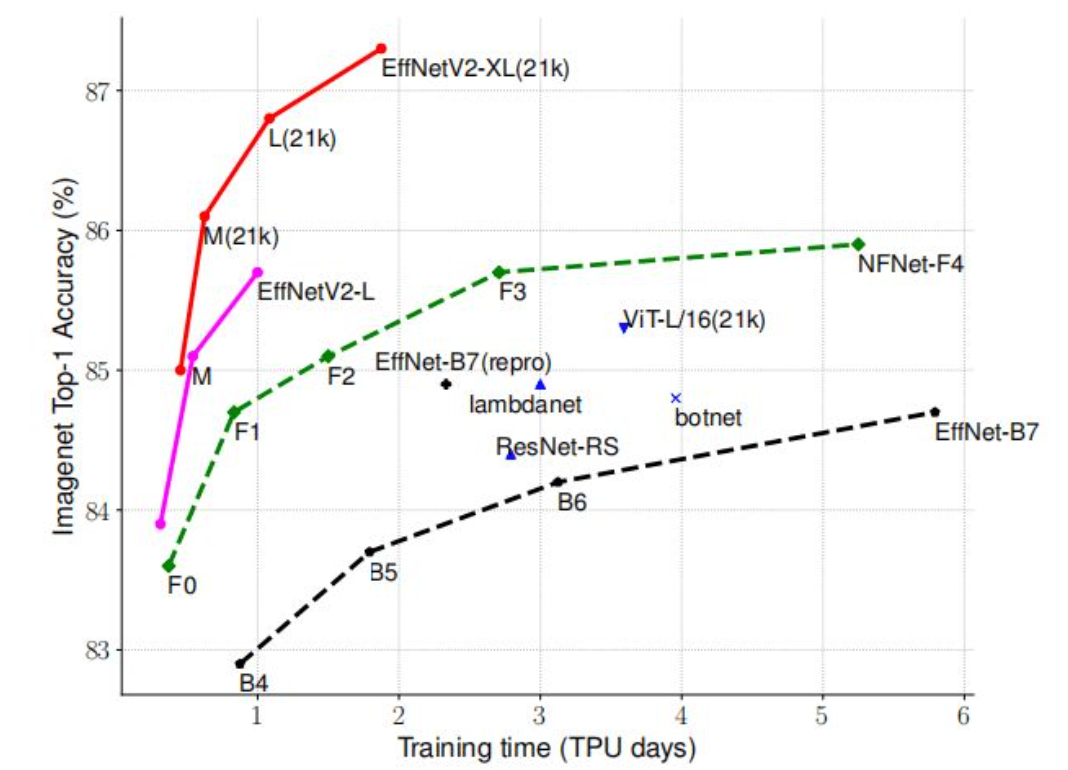
\includegraphics[width=0.6\textwidth]{picture/efficientnet.png}
	\caption{ImageNet ILSVRC2012 top-1 Accuracy vs. Training Time and Parameters}
\end{figure}

原论文中采用NAS搜索技术(trainning-aware NAS framework),以准确率,参数效率,
训练效率三个维度为优化目标,搜索得到了如下 EfficientNetV2-S 模型框架
\footnote{注:本文在实践过程中主要基于 EfficientNetV2-S 网络框架,因此本文不涉及对
EfficientNetV2-M,EfficientNetV2-L模型的探讨。}
\begin{table}[H]
    \centering
    \caption{EfficientNetV2-S architecture}
    \begin{tabular}{ccccc}
    \hline
        Stage & Operator & Stride & \#Channels & \#Layers \\ \hline
        0 & Conv3x3 & 2 & 24 & 1 \\ 
        1 & Fused-MBConv1, k3x3  & 1 & 24 & 2 \\ 
        2 & Fused-MBConv4, k3x3 & 2 & 48 & 4 \\ 
        3 & Fused-MBConv4, k3x3  & 2 & 64 & 4 \\ 
        4 & MBConv4, k3x3, SE0.25 & 2 & 128 & 6 \\ 
        5 & MBConv6, k3x3, SE0.25  & 1 & 160 & 9 \\ 
        6 & MBConv6, k3x3, SE0.25 & 2 & 256 & 15 \\ 
        7 & Conv1x1 \& Pooling \& FC & - & 1280 & 1 \\ \hline
    \end{tabular}
\end{table}
\begin{itemize}
	\item $\#$Layers 表示该 Stage 重复堆叠 Operator 的次数。Stride 表示该 Stage 第一个 
	Opertator 模块的步距,$\#$Channels 表示该 Stage 输出的特征矩阵的 Channels。
	\item Conv3x3 代表普通的 3*3 卷积网络 + SiLU 激活函数 + BN 层(Batch Normalization)。
	\item Fused-MBConv 模块如图 5 所示,值得注意的是,这里的 Dropout 层
	\footnote{原论文:[1603.09382] Deep Networks with Stochastic Depth (arxiv.org)}
	为 Stochastic Depth,会随机丢掉整个 block 的主分支。
\end{itemize}
\begin{figure}[H]
	\centering
	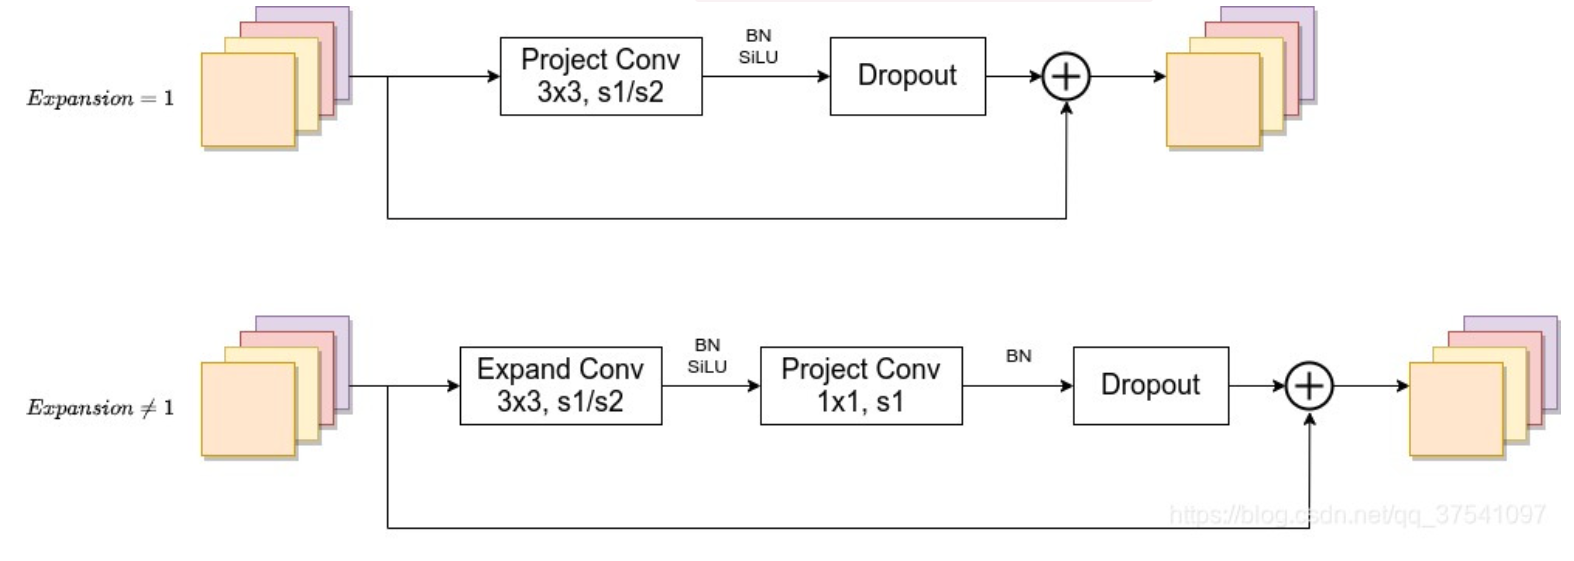
\includegraphics[width=0.8\textwidth]{picture/fused-mbconv.png}
	\caption{Fused-MBConv 模块}
\end{figure}
\begin{figure}[H]
	\centering
	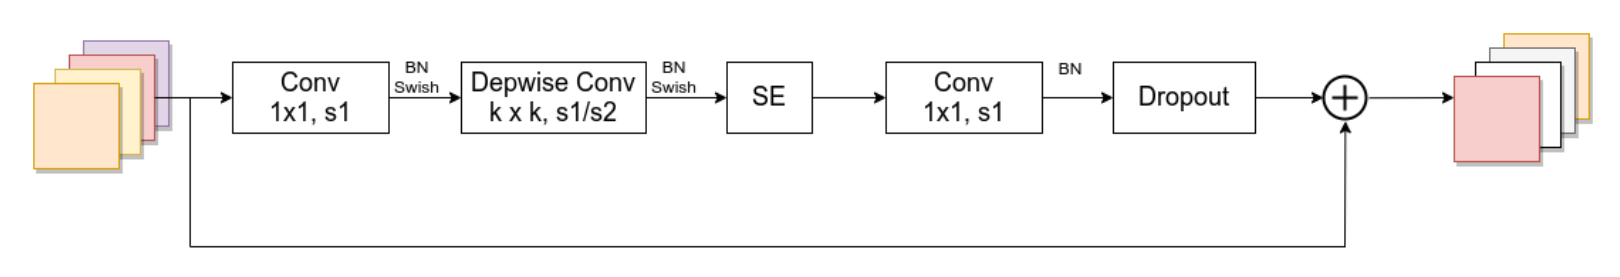
\includegraphics[width=0.8\textwidth]{picture/mbconv.png}
	\caption{MBConv 模块}
\end{figure}


\section{实验结果与分析}
\subsection{简单卷积网络}
由于数据量较少,为了避免发生过拟合,本小组记录了不同 epoch 下测试集的准确率:
\begin{figure}[H]
	\centering
	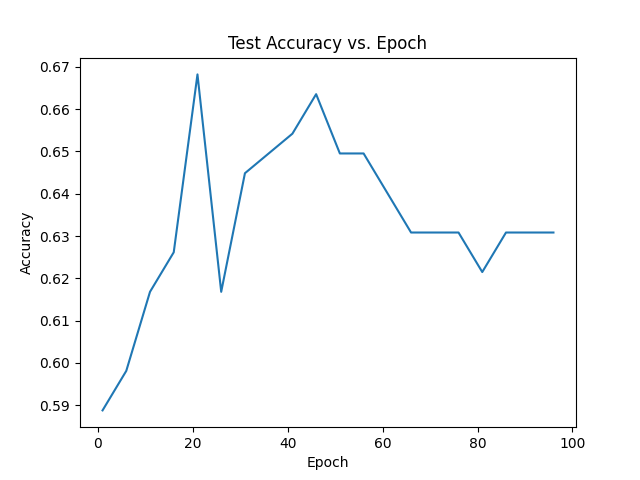
\includegraphics[width=0.6\textwidth]{picture/simplecnn.png}
	\caption{SimpleCNN Accuracy vs. Epoch}
\end{figure}
可以看到,在 20 个 epoch 之后,简单卷积网络的测试集准确率达到了 0.67 左右,此后准确率
下降后趋于稳定。因此,在之后的训练过程中,本小组选择了 20 个 epoch 作为训练次数。

尽管本地测试的准确率可达 0.67,但在 HRDC 平台上的分数并不理想,仅为 0.38。因此,在此
基础上,本小组引入了图像的预处理,最终本地测试的准确率达到了 0.71,HRDC 平台上的分数
也有所提升,达到了 0.41。考虑到是否对图像压缩的过于的小,本小组在之后的训练中对图像
的尺寸进行了调整,将图像的大小调整为 300*300,然而无论是本地测试的准确率还是 HRDC 
平台上的分数甚至有所下降。本小组猜测可能是过拟合的问题。
\begin{table}[H]
    \centering
    \begin{tabular}{|c|c|c|c|}
    \hline
    preprocess & input size & local accuracy & HRDC score \\
    \hline
    - & 64*64 & 0.67 & 0.38 \\
	1 & 64*64 & 0.71 & 0.41 \\
	1 & 300*300 & 0.64 & 0.35 \\
    \hline
    \end{tabular}
    \caption{SimpleCNN Experiment Results}
\end{table}

对于本地测试的准确率与 HRDC 平台上的分数差距较大的问题,本小组在研究了 HRDC 平台的
评分标准后发现,HRDC 平台上的分数由三项指标决定,分别为 Kappa、F1 和 Specificity,
即与随机分类器的一致性、召回率和负样本的识别率。本小组发现,简单卷积网络在 HRDC 的
前两项指标表现极差,导致了最终的分数较低。

通过输出 0 和 1 的召回率,本小组发现简单卷积网络对于 0 的召回率较高,但对于 1 的召回率
较低,本小组初步认为是由于数据集中 0 的数量远远大于 1 的数量,导致了模型对于 0 的识别
更为准确。然而在减少了 0 的数量后,模型的准确率反而下降,1 的召回变为 100\%,暂未发现
原因。因此,本小组认为简单卷积网络在高血压视网膜病变分类任务上具有一定的效果,但仍
存在一些问题,需要进一步优化。

\subsection{ResNet}
在 Resnet 模型上,对数据进行简单的预处理,将输入图像尺寸统一为 $256\times 256$,并随机旋转
下,经过 50 个 epoch 训练之后,在本地训练集和测试集上的正确率分别达到了 0.93 和 0.66。在 HRDC
平台上的分数平均为 0.54,
\begin{table}[H]
    \centering
    \begin{tabular}{|l|l|l|l|}
    \hline
        Kappa & F1 Score & Specificity & Average \\ \hline
        0.32 & 0.67 & 0.64 & 0.54 \\ \hline
    \end{tabular}
    \caption{Resnet Experiment Result}
    \label{Resnet Experiment Result}
\end{table}
但是相比于 resnet,EfficientNet 使用了一种称为 Compound Scaling 的方法,通过在网络
的深度、宽度和分辨率上进行统一的缩放来设计网络结构,从而在不同的模型大小之间实现了平衡。
在相同计算资源下通常能够达到比 ResNet 更好的性能,所以本小组决定采用效果更好 EfficientNet.

\subsection{EfficientNetV2}
在 EfficientNetV2 模型上,本小组尝试了不同的数据增强方法,包括 CLAHE、CLAHE+CutMix 及
不同预处理方法的组合。以下为不同数据增强方法的实验结果:
\begin{table}[H]
    \centering
    \begin{tabular}{|c|c|c|c|c|c|}
    \hline
        输入尺寸 & 数据增强方法 & Kappa & F1 & Specificity & Average(Score)\\
    \hline
		224*224 & - & 0.21 & 0.51 & 0.71 & 0.48 \\
        300*300 & - & 0.31 & 0.54 & 0.82 & 0.56 \\
        300*300 & CLAHE 	& \textbf{0.42} & \textbf{0.60} & 0.87 & \textbf{0.63} \\
        300*300 & CLAHE +CutMix & 0.26 & 0.45 & \textbf{0.89} & 0.54\\
        300*300 & 去掉去噪 & 0.23 & 0.60 & 0.44 & 0.42 \\
        300*300 & 去掉最后两步 & 0.20 & 0.49 & 0.73 & 0.47 \\
    \hline
	\end{tabular}
	\caption{EfficientNetV2 Experiment Results}
\end{table}
可以看到,在输入图像尺寸为 300*300 的情况下,运用 CLAHE 数据增强方法得到的效果最好,
而非简单卷积网络模型实验中采用全部预处理方法的效果最好。本小组由此推断,在不同的模型上,
不同的数据预处理方法可能会有不同的效果,因此在实际应用中需要根据具体情况进行选择。
在此训练模式下,损失函数输出和准确率随训练次数的变化如下图所示:
\begin{figure}[H]
	\centering
	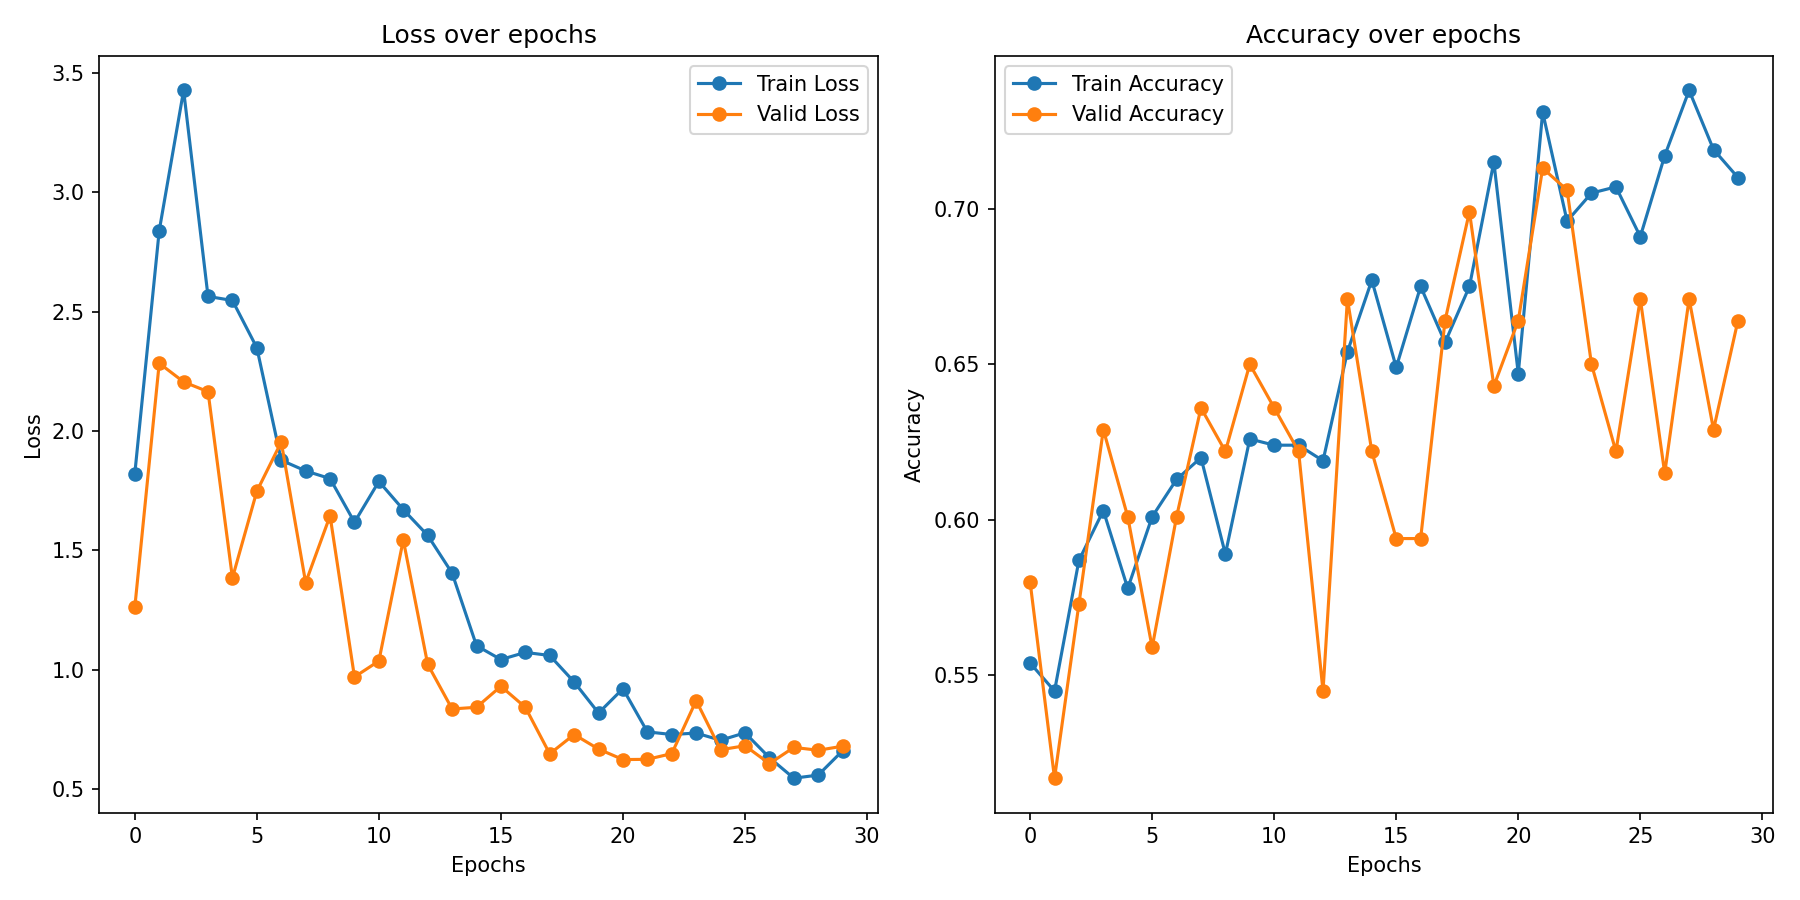
\includegraphics[width=0.8\textwidth]{picture/efficientnet-epoch.png}
	\caption{EfficientNetV2 Loss and Accuracy vs. Epoch}
\end{figure}

最后,由于三种模型的分数差距较大,EfficientNetV2 模型的分数远高于其他两种模型,因此,
本小组放弃采用投票的方式,直接选择了 EfficientNetV2 模型作为最终的模型。
\section{特色与创新}
本文在高血压视网膜病变分类任务中,尝试了不同的数据预处理方法和深度学习模型,通过对比
实验结果,发现了不同模型和数据预处理方法之间的优劣势,为后续的研究和实践提供了一定的
参考。

在数据预处理方面,本小组尝试了 CLAHE、CutMix 等方法,发现 CLAHE 方法在高血压视网膜病变
分类任务中具有较好的效果,能够有效提高图像的质量和清晰度,有助于提取图像的特征和信息。

在模型选择方面,在传统的二分类模型 ResNet 外,本小组还创新性地尝试了 EfficientNetV2 模型,
发现该模型在高血压视网膜病变分类任务中具有较好的性能,能够有效提高模型的准确率和泛化能力,
有助于提高模型的分类效果和稳定性。

\begin{thebibliography}{9}
	\bibitem{ref1}
	EfficientNetV2: Smaller Models and Faster Training, Mingxing Tan, Quoc V. Le
	\bibitem{ref2}
	Deep Networks with Stochastic Depth, Gao Huang, Yu Sun, Zhuang Liu, Daniel Sedra, Kilian Weinberger
	\bibitem{ref3}
	EfficientNet: Rethinking Model Scaling for Convolutional Neural Networks, Mingxing Tan, Quoc V. Le
	\bibitem{ref4}
	Contrast Limited Adaptive Histogram Equalization, K. Zuiderveld
	\bibitem{ref5}
	CutMix: Regularization Strategy to Train Strong Classifiers with Localizable Features, Sangdoo Yun, Dongyoon Han, Seong Joon Oh, Sanghyuk Chun, Junsuk Choe, Youngjoon Yoo
	\bibitem{ref6}
	基于深度卷积集成网络的视网膜多种疾病筛查和识别方法, 王禾扬, 杨启鸣, 朱旗
	\bibitem{ref7}
	Automated Hypertensive Retinopathy Detection from Fundus Retinal Images, Syed Nakib Hossain, Shamman Noor, Raufur Rahman Khan, Prottay Debnath, Shafi Uddin Siddique,
Kazi Rezaul Karim
\end{thebibliography}

\end{document}
